\documentclass[11pt, a4paper]{article}

\usepackage[margin=2.0cm, top=1.8cm, bottom=1.8cm]{geometry}
\usepackage{hyperref}
\usepackage{booktabs}
\usepackage{array}
\usepackage{xcolor}
\usepackage{enumitem}
\usepackage{titlesec}
\usepackage{tikz}
\usetikzlibrary{positioning, arrows.meta, shapes.geometric, fit, backgrounds}

\hypersetup{
    colorlinks=true,
    linkcolor=blue!50!black,
    urlcolor=blue!50!black,
}

\titleformat{\section}{\large\bfseries}{\thesection}{0.6em}{}
\titlespacing*{\section}{0pt}{1.2ex}{0.5ex}
\titleformat{\subsection}{\normalsize\bfseries}{\thesubsection}{0.5em}{}
\titlespacing*{\subsection}{0pt}{0.9ex}{0.3ex}

\setlist[itemize]{itemsep=0.2ex, topsep=0.4ex, leftmargin=*}
\setlist[enumerate]{itemsep=0.2ex, topsep=0.4ex, leftmargin=*}

\setlength{\parskip}{0.4ex}
\setlength{\parindent}{0pt}
\renewcommand{\arraystretch}{1.12}

\title{\vspace{-2.0cm}\textbf{DementiaNext --- Companion Chatbot (Patient \& Caregiver)}}
\author{}
\date{}

\begin{document}
\maketitle
\vspace{-1.4cm}

\section{Overview}

The Companion Chatbot is a dual-mode conversational agent embedded in the DementiaNext platform. It serves two distinct audiences from a shared underlying infrastructure:

\begin{itemize}
    \item \textbf{Patient mode} --- a calming, validation-therapy-oriented companion for the person living with dementia. It uses Naomi Feil's Validation Therapy and Reminiscence Therapy techniques, never corrects or quizzes the patient, and adapts language complexity to the patient's clinical stage (mild / moderate / severe).
    \item \textbf{Caregiver mode} --- a clinical advisor for family caregivers and care staff. It provides evidence-grounded answers on dementia subtypes, medication interactions, behavioral management protocols (sundowning, agitation, wandering), and emergency triage criteria such as FAST stroke recognition.
\end{itemize}

Both modes share the same Django backend, the same Llama-3.3-70B model served through the Groq Inference API, and the same retrieval-augmented generation (RAG) layer. They differ in three deliberate places: the system prompt template, the RAG collection consulted, and the per-patient context injected at request time. The system is grounded in a curated 10-file knowledge base spanning dementia stages, pharmacology, behavioral management, communication therapy, caregiver protocols, and detailed neurological subtype information.

\section{Pipeline Diagram}

\begin{center}
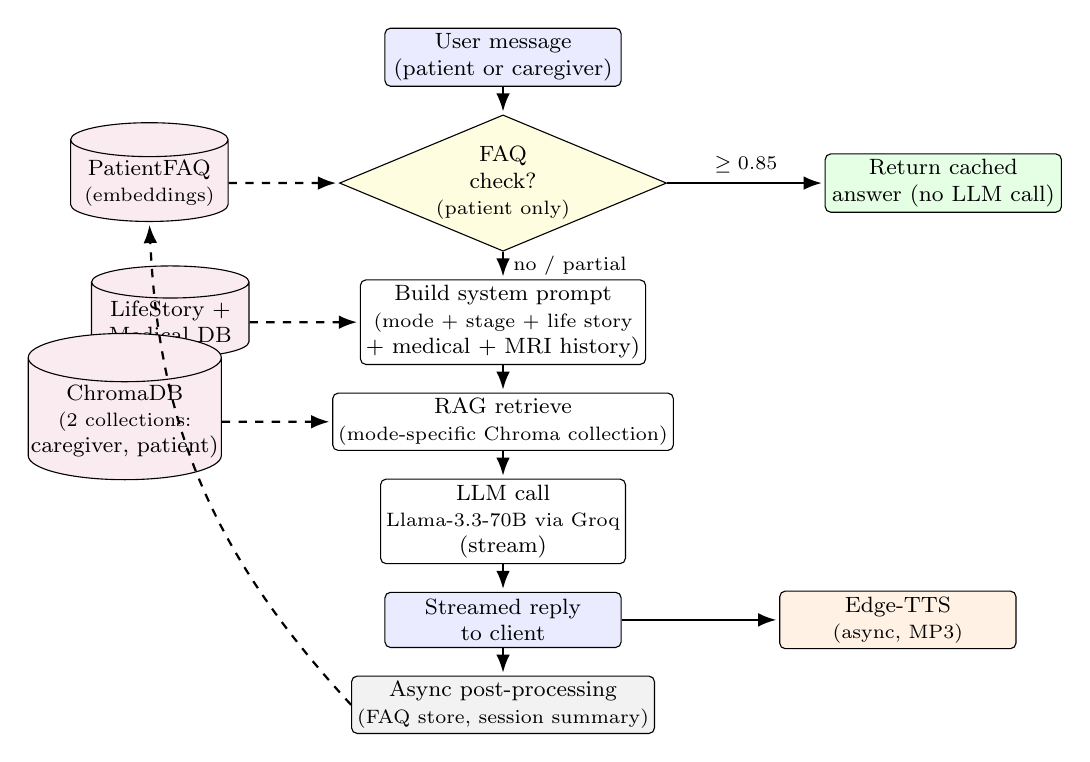
\begin{tikzpicture}[
    node distance=3.5mm and 6mm,
    every node/.style={font=\footnotesize},
    box/.style={rectangle, draw, rounded corners=2pt, minimum height=7mm, minimum width=30mm, align=center, inner sep=2pt},
    decision/.style={diamond, draw, aspect=2.4, inner sep=1pt, align=center},
    store/.style={cylinder, draw, shape border rotate=90, aspect=0.25, minimum height=8mm, minimum width=20mm, align=center, inner sep=1pt},
    arrow/.style={-Latex, thick, shorten >=1pt},
    dashedarrow/.style={-Latex, dashed, thick, shorten >=1pt},
]
    % --- main flow ---
    \node[box, fill=blue!8] (user) {User message\\(patient or caregiver)};
    \node[decision, fill=yellow!12, below=of user] (faq) {FAQ\\check?\\\scriptsize(patient only)};
    \node[box, fill=green!10, right=20mm of faq] (cached) {Return cached\\answer (no LLM call)};
    \node[box, below=of faq] (ctx) {Build system prompt\\\scriptsize(mode + stage + life story\\+ medical + MRI history)};
    \node[box, below=of ctx] (rag) {RAG retrieve\\\scriptsize(mode-specific Chroma collection)};
    \node[box, below=of rag] (llm) {LLM call\\\scriptsize Llama-3.3-70B via Groq\\(stream)};
    \node[box, fill=blue!8, below=of llm] (resp) {Streamed reply\\to client};
    \node[box, fill=orange!10, right=20mm of resp] (tts) {Edge-TTS\\\scriptsize(async, MP3)};
    \node[box, fill=gray!10, below=of resp] (post) {Async post-processing\\\scriptsize(FAQ store, session summary)};

    % --- data stores ---
    \node[store, fill=purple!8, left=14mm of faq] (faqdb) {PatientFAQ\\\scriptsize(embeddings)};
    \node[store, fill=purple!8, left=14mm of ctx] (lstore) {LifeStory +\\Medical DB};
    \node[store, fill=purple!8, left=14mm of rag] (chroma) {ChromaDB\\\scriptsize(2 collections:\\caregiver, patient)};

    % --- arrows ---
    \draw[arrow] (user) -- (faq);
    \draw[arrow] (faq) -- node[above, font=\scriptsize]{$\geq 0.85$} (cached);
    \draw[arrow] (faq) -- node[right, font=\scriptsize]{no / partial} (ctx);
    \draw[arrow] (ctx) -- (rag);
    \draw[arrow] (rag) -- (llm);
    \draw[arrow] (llm) -- (resp);
    \draw[arrow] (resp) -- (post);
    \draw[arrow] (resp) -- (tts);

    \draw[dashedarrow] (faqdb) -- (faq);
    \draw[dashedarrow] (lstore) -- (ctx);
    \draw[dashedarrow] (chroma) -- (rag);
    \draw[dashedarrow] (post.west) to[bend left=20] (faqdb.south);

\end{tikzpicture}
\end{center}

\textit{Solid arrows: control flow. Dashed arrows: data dependency. The FAQ short-circuit (top-right) returns a stored answer without invoking the LLM when a previous question matches with cosine similarity $\geq 0.85$ --- a clinically motivated mechanism that ensures dementia patients receive identical phrasing across repeated queries.}

\section{Data Model}

Five Django models support the companion. They are stored in the shared Postgres database alongside detection and authentication data.

\begin{center}
\small
\begin{tabular}{>{\bfseries}p{3.5cm} p{12.6cm}}
\toprule
Model & Purpose \\
\midrule
\texttt{LifeStoryEntry} & Per-patient autobiographical content used for personalized responses and reminiscence therapy. Eight categories (family, daily routine, favorites, memories, places, health, people, instructions). Supports text and voice entries with transcripts; emotional valence flag (positive / neutral / sensitive); priority field for conflict resolution; trigger questions for direct Q\&A matching. \\
\texttt{ConversationSession} & Per-conversation envelope; tracks mode, start/end times, message count, cognitive stage at the time of conversation, and an LLM-generated summary used for session-to-session continuity. \\
\texttt{ConversationMessage} & Individual user / assistant / system messages within a session, with optional audio URL and per-message latency in milliseconds. \\
\texttt{PatientFAQ} & Frequently-repeated patient questions paired with consistent canonical answers. Stores a pickled sentence-transformer embedding to avoid recomputing at every match query (saves $\sim$200 ms per request). \\
\texttt{PatientCompanionConfig} & Per-patient settings: cognitive stage, preferred TTS voice, language, life-story enablement, consent metadata. \\
\bottomrule
\end{tabular}
\end{center}

\section{Component Implementation}

\subsection{Mode-Aware RAG (\texttt{rag\_engine.py})}

The retrieval layer uses ChromaDB as a persistent vector store with a sentence-transformers embedding function (\texttt{all-MiniLM-L6-v2}, 384-dim). At startup the engine ingests the 10-file curated knowledge base, splits each file into overlapping paragraph-aligned chunks, and indexes them into \textbf{two separate collections}:

\begin{itemize}
    \item \textbf{Caregiver collection} --- all 10 knowledge files; chunk size 800 tokens, overlap 100, $n=8$ retrievals per query. Optimized for clinical depth.
    \item \textbf{Patient collection} --- only 4 files (dementia stages, communication therapy, patient-specific scenarios, emotional support); chunk size 400, overlap 60, $n=3$ retrievals. Optimized for short, soothing context fragments.
\end{itemize}

A SHA-256 content hash is stored on each collection's metadata; if the underlying \texttt{.txt} files change, the affected collection is rebuilt automatically on the next request. Retrieved passages are formatted differently depending on mode --- caregiver mode receives the passages with a "base your answers on this material only" preamble, while patient mode receives them as internal behavioral guidance with explicit instructions never to quote them verbatim to the patient.

\subsection{FAQ Detector (\texttt{faq\_detector.py})}

For the patient mode, dementia clinical practice recommends answering repeated questions with identical wording each time. The FAQ detector implements this:

\begin{enumerate}
    \item Encode the patient's question into a 384-dim normalized embedding (sentence-transformers, lazy-loaded).
    \item Load up to 50 most-asked stored FAQs for this patient. For each, deserialize the pickled embedding from the \texttt{question\_embedding} BLOB column. Newly-stored FAQs without embeddings are computed in batch and persisted back to the row.
    \item Compute cosine similarity in a single NumPy dot-product against the full FAQ matrix. Take the top-1 match.
    \item Apply two thresholds: similarity $\geq 0.85$ returns the stored answer verbatim and bypasses the LLM entirely (zero-latency response, zero token cost); similarity $\geq 0.60$ injects the prior question/answer pair into the system prompt as soft context for the LLM to mimic.
\end{enumerate}

The FAQ store is updated asynchronously after each LLM-generated response so the request thread is not blocked.

\subsection{Context Builder (\texttt{context\_builder.py})}

Constructs the system prompt for each LLM call. It assembles seven sections: patient demographics, current medications and allergies, medical history, the most recent MRI detection results from the \texttt{detection} app, the life-story summary grouped by category and emotional valence, the previous-session summaries (last three sessions for patient-mode continuity), and the FAQ context. The prompt template is selected by mode and parameterized by cognitive stage, with stage-specific behavioral rules (e.g., 5--8 word maximum for the severe stage, anchor phrases involving the patient's name).

\subsection{Conversation Engine (\texttt{conversation\_engine.py})}

Orchestrates the request: FAQ short-circuit $\to$ context build $\to$ RAG retrieval $\to$ Groq streaming chat completion $\to$ response persistence. Per-mode generation parameters: temperature $0.7$ and 400 tokens for patient (warmer, more variable), temperature $0.4$ and 500 tokens for caregiver (more deterministic and detailed). Post-processing (FAQ insertion, session summary generation every 10 messages) runs in a daemon thread so the user-perceived response time only includes the FAQ check, prompt build, and LLM stream.

\subsection{TTS Layer (\texttt{tts\_service.py})}

The patient interface supports speech output through Microsoft Edge's free TTS service via the \texttt{edge-tts} library. Synthesis is launched in a background thread and exposed through a task-id polling API so the chat reply can stream to the user immediately while the audio MP3 is generated alongside. The patient's preferred voice (default \texttt{en-US-AriaNeural}) is configurable per-patient through \texttt{PatientCompanionConfig}.

\section{Personalization and Safety}

\textbf{Personalization} is grounded in three patient-specific information sources injected at every prompt build: the life-story corpus, the patient's medical record (medications, allergies, history), and the latest MRI detection results. The result is that the same generic Llama-3.3-70B model produces materially different responses for different patients --- referencing their actual relatives, hometown, occupation, and clinical history.

\textbf{Safety} is enforced at multiple layers: explicit anti-hallucination rules in the system prompt forbid invented names, dosages, or care protocols; the caregiver mode mandates "discuss with the doctor" responses for medication changes and emergency-pattern recognition for FAST stroke criteria; sensitive life-story entries (e.g., bereavements) are flagged so the LLM avoids triggering distress; and the patient mode is explicitly instructed never to correct, quiz, or reinforce dangerous delusions (such as a patient wanting to drive).

\section{Performance Characteristics}

\begin{center}
\small
\begin{tabular}{>{\raggedright\arraybackslash}p{6.0cm} >{\raggedleft\arraybackslash}p{2.8cm} >{\raggedright\arraybackslash}p{6.5cm}}
\toprule
\textbf{Path} & \textbf{Latency} & \textbf{Notes} \\
\midrule
FAQ exact match (cached answer) & $\sim$50--150 ms & query embedding + dot-product only \\
Cold first message in session & $\sim$2.0--2.5 s & includes RAG warm-up if Chroma not yet loaded \\
Warm streaming response & $\sim$0.6--1.2 s to first token & Llama-3.3-70B on Groq \\
Edge-TTS synthesis (asynchronous) & $\sim$1--3 s & does not block reply \\
Session summary regeneration & every 10 msgs & runs in daemon thread \\
\bottomrule
\end{tabular}
\end{center}

\section{Conclusion}

The Companion Chatbot is the most user-facing component of DementiaNext and the place where clinical specificity makes the largest difference between a generic LLM-wrapper and a useful tool. Its architecture --- dual-mode prompts, mode-aware RAG, per-patient FAQ caching, life-story grounding, and stage-adaptive language complexity --- is built to satisfy two distinct workflows from a shared substrate: a soothing, repetition-tolerant companion for the patient, and a clinically rigorous advisor for the caregiver. The system is implemented entirely in open libraries (Django, ChromaDB, sentence-transformers, edge-tts, the Groq SDK) and runs on the same free-tier Hugging Face Space as the rest of the backend, with no additional infrastructure.

\end{document}
